\label{ch:compressible-theory}


%-----------------------------------------------------------------------------
\section{Euler equation properties}

The Euler equations\footnote{ We focus on the Euler equations, which
are the most commonly modeled set of fluid equations in astrophysics.
The more general equation set, the Navier-Stokes equations, includes
dissipative terms.  However, for astrophysical flows, the scales on
which these dissipative terms operate are usually much smaller than
the system of interest (equivalently, Reynolds numbers of
astrophysical flows are very large).} describe conservation of 
mass, momentum, and energy in the fluid approximation.  Their general
form, without any source terms, is:  \MarginPar{need to add a discussion of the N-S equations and dimensionless numbers}
\begin{align}
\ddt{\rho} + \nabla \cdot (\rho \Ub) &= 0 \\
\ddt{(\rho \Ub)} + \nabla \cdot (\rho \Ub \Ub) + \nabla p &= 0 \\
\ddt{(\rho E)} + \nabla \cdot (\rho E \Ub + p \Ub ) &= 0 
\end{align}
Here $\rho$ is the density, $\Ub$ is the velocity vector, $\Ub =
u\hat{x} + v\hat{y}$, $p$ is the pressure, and $E$ is the total energy
/ mass, and can be expressed in terms of the specific internal energy,
$e$, and kinetic energy as:
\begin{equation}
E = e + \frac{1}{2} |\Ub|^2
\end{equation}
The equations are closed with the addition of an equation of state.  A common
choice is the gamma-law EOS:
\begin{equation}
p = \rho e(\gamma - 1)
\end{equation}
where $\gamma$ is the ratio of specific heats for the gas/fluid (for
an ideal, monatomic gas, $\gamma = 5/3$), but any relation of the form
$p = p(\rho, e)$ will work.

For a derivation of the equations of hydrodynamics using moments of
the Boltzmann equation see \cite{shu,choudhuri}.  For a
physically-motivated derivation from conservation, see \cite{leveque:2002}.

In one dimension, they appear as\footnote{assuming Cartesian coordinates}:
\begin{align}
\frac{\partial \rho}{\partial t} +
    \frac{\partial (\rho u)}{\partial x} &= 0 \\
%
\frac{\partial(\rho u)}{\partial t} +
    \frac{\partial (\rho uu + p)}{\partial x} &= 0 \\
%
\frac{\partial(\rho E)}{\partial t} +
    \frac{\partial(\rho u E + u p)}{\partial x} &= 0
\end{align}

One thing that we can notice immediately is that there is no need for
temperature in this equation set, although often, when source terms
are present, we will need to obtain temperature from the equation of
state.

In this form, the equations are said to be in {\em conservative form},
i.e.\ they can be written as:
\begin{equation}
\Uc_t + \left [\Fb(\Uc) \right ]_x = 0
\end{equation}
with
\begin{equation}
\Uc = \left ( \begin{array}{c} \rho \\ \rho u \\ \rho E \end{array} \right )
%
\qquad
%
\Fb(\Uc) = \left ( \begin{array}{c} \rho u \\ \rho uu + p \\ \rho u E + up \end{array} \right )
\end{equation}
%
We can write this in {\em quasi-linear} form by first expressing the
flux vector in terms of the conserved variables directly.  Taking $m
\equiv \rho u$, $\mathcal{E} \equiv \rho E$, and assuming a gamma-law
EOS%
\footnote{we can relax this assumption by writing $p = p(\rho, e)$, and then
taking the derivatives of this as needed:  $\partial p/\partial \rho$, 
$\partial p/\partial m = \partial p /\partial e|_\rho \partial e/\partial m$,
and $\partial p/\partial \mathcal{E} = \partial p/\partial e|_\rho \partial e/\partial \mathcal{E}$,
with $e = (\mathcal{E} - \myhalf m^2/\rho)/\rho$.  But as we'll see, there are
simpler systems to work with.},
\begin{equation}
p = \rho e (\gamma-1) =  \left (\mathcal{E} - \frac{1}{2} \frac{m^2}{\rho}\right )(\gamma - 1)
\end{equation}
we have
\begin{equation}
\Fb(\Uc) = \left ( \begin{array}{c}
      m \\
      \frac{1}{2}\frac{m^2}{\rho} \left (3 - \gamma \right ) +
          \mathcal{E} (\gamma - 1) \\
      \frac{m\mathcal{E}}{\rho} \gamma -\frac{1}{2} \frac{m^3}{\rho^2} (\gamma -1) \end{array} \right )
\end{equation}
The Jacobian%
\footnote{
The Jacobian, ${\bf J}$ of a vector $\Fb(\Uc)$ with $\Fb = (f_1, f_2, \ldots, f_n)^\intercal$ and
$\Uc = (u_1, u_2, \ldots, u_n)^\intercal$ is 
\begin{equation*}
{\bf J} \equiv \frac{\partial \Fb}{\partial \Uc} = \left (
  \begin{array}{cccc}
     \partial f_1/\partial u_1 & \partial f_1/\partial u_2 & \ldots & \partial f_1/\partial u_n \\
     \partial f_2/\partial u_1 & \partial f_2/\partial u_2 & \ldots & \partial f_2/\partial u_n \\
     \vdots                    & \vdots                    & \ddots & \vdots \\
     \partial f_n/\partial u_1 & \partial f_n/\partial u_2 & \ldots & \partial f_n/\partial u_n 
  \end{array} \right )
\end{equation*}
}
of this flux vector can now be computed as $\Ab = \partial
\Fb/\partial \Uc$:
\begin{equation}
\Ab(\Uc) = \left ( \begin{array}{ccc}
   0  & 1 & 0 \\
   -\frac{1}{2}u^2(3 -\gamma) & u (3 -\gamma) & \gamma - 1 \\
   \frac{1}{2}(\gamma -2)u^3 - \frac{uc^2}{\gamma -1} &
       \frac{3-2\gamma}{2} u^2 + \frac{c^2}{\gamma -1} & u \gamma
  \end{array} \right )
\end{equation}\MarginPar{SymPy notebook?}
where the speed of sound is $c = \sqrt{\gamma p/\rho}$.   With this, our
system can be written as:
\begin{equation}
\Uc_t + \Ab(\Uc) \Uc_x = 0
\end{equation}
This matrix is quite complex and difficult to work with.  The
eigenvectors of this matrix can be found in a variety of sources
(e.g. \cite{toro:1997,athena}).


An alternate way to express these equations is using the {\em
  primitive variables}: $\rho, u, p$.
\begin{exercise}[Primitive variable form of the Euler equations]
{Show that the Euler equations in primitive form can
  be written as
\begin{align}
\ddt{\rho} + u \ddx{\rho} + \rho \ddx{u} &= 0 \\
\ddt{u} + u \ddx{u} + \frac{1}{\rho} \ddx{p} &= 0 \\
\ddt{p} + u \ddx{p} + \gamma p \ddx{u} &= 0
\end{align}
}
\end{exercise}
Notice that the velocity equation looks like Burgers' equation, and 
is nonlinear.  This nonlinearity will admit shock and rarefaction
solutions like we saw with Burgers' equation.

%
The primitive variable system can be written compactly as:
\begin{equation}
\qb_t + \Ab(\qb) \qb_x = 0
\end{equation}
where
\begin{equation}
\qb = \left ( \begin{array}{c} \rho \\ u \\ p \end{array} \right )
%
\qquad
\Ab(\qb) = \left ( \begin{array}{ccc} u  & \rho     & 0 \\
                                  0  &  u       & 1/\rho \\
                                  0  & \gamma p & u \end{array} \right )
\label{eq:primitivesystem}
\end{equation}



The eigenvalues of $\Ab$ can be found via $| \Ab - \lambda {\bf I} | = 0$,
where $|\ldots|$ indicates the determinant and $\lambda$ are the eigenvalues.
\begin{exercise}[The eigenvalues of the Euler system]
{
Show that the eigenvalues of $\Ab$ are $\lambda^\evm = u -c$, $\lambda^\evz = u$, $\lambda^\evp = u+c$.
}
\end{exercise}
Note that both the conserved Jacobian matrix, $\Ab(\Uc)$, and the
primitive variable matrix, $\Ab(\qb)$, have the same eigenvalues,
 since they represent the same physics.

In Eq.~\ref{eq:primitivesystem}, we used the algebraic gamma-law
equation of state to replace $e$ with $p$, however, for a general
equation of state, we can get the appropriate expression by writing $p
= p(\rho, s)$:
\begin{equation}
\frac{Dp}{Dt} = \left . \frac{\partial p}{\partial \rho} \right |_s
     \frac{D\rho}{Dt} +
     \left . \frac{\partial p}{\partial s} \right |_\rho
     \cancelto{0}{\frac{Ds}{Dt}}
\end{equation}
where $Ds/Dt = 0$ when no entropy sources are present (we will relax this
assumption in \S~\ref{ch:lm:constraints}).  Recognizing
that $\Gamma_1 \equiv \partial \log p/\partial \log \rho |_s$, we have:
\begin{equation}
\frac{\partial p}{\partial t} + u \frac{\partial p}{\partial x}
  + \Gamma_1 p \frac{\partial u}{\partial x} = 0  \label{eq:euler:pgeneral}
\end{equation}
as the generalization of the pressure equation\footnote{$\Gamma_1$ is one of the
many adiabatic indices that describe the coupling between different
thermodynamic quantities under compression/expansion.  Any stellar structure
book should give a good background, e.g., \cite{HKT}.  Note that for an ideal gas, $\Gamma_1 = \gamma$}.
The sound speed is then $c^2 = \Gamma_1 p /\rho$.

These eigenvalues are the speeds at which information propagates
through the fluid.  Since the eigenvalues are real, this system (the
Euler equations) is said to be {\em hyperbolic}.  Additionally, since
$\Ab = \Ab(\qb)$, the system is said to be {\em quasi-linear}.  Note,
physically, these eigenvalues are telling us that information is
communicated at the speed of the fluid ($u$), as well as the speed of
sound moving with respect to the fluid ($u \pm c$).

We'll use the symbols $\{-,\circ,+\}$ to denote the eigenvalues and their
corresponding eigenvectors throughout these notes.
%
The right and left eigenvectors can be found via:
\begin{equation}
\Ab \, \rb^\enu = \lambda^\enu \rb^\enu \; ;
\qquad
\lb^\enu \, \Ab  = \lambda^\enu \lb^\enu
\end{equation}
where $\nu = \{-,\circ,+\}$ corresponding to the three waves, and
there is one right and one left eigenvector for each of the eigenvalues.
%
\begin{exercise}[Eigenvectors of the Euler system]
{
Show that the right eigenvectors are:
\begin{equation}
\label{eq:euler:primRevs}
\rb^\evm = \left ( \begin{array}{c} 1 \\ -c/\rho \\ c^2 \end{array} \right )
%
\qquad
\rb^\evz = \left ( \begin{array}{c} 1 \\ 0 \\ 0  \end{array} \right )
%
\qquad
\rb^\evp = \left ( \begin{array}{c} 1 \\ c/\rho \\ c^2 \end{array} \right )
\end{equation}
and the left eigenvectors are:
\begin{align}
\lb^\evm &= \left ( \begin{array}{ccc} 0 & -\frac{\rho}{2c} & \frac{1}{2c^2}
                  \end{array} \right ) \\
%
\qquad
\lb^\evz &= \left ( \begin{array}{ccc} 1 & 0 & -\frac{1}{c^2}  \end{array} \right ) \\
%
\qquad
\lb^\evp &= \left ( \begin{array}{ccc} 0 & \phantom{+}\frac{\rho}{2c} & \frac{1}{2c^2} \end{array} \right )
\end{align}
Note that in general, there can be an arbitrary constant in front of each
eigenvector.  Here they are normalized such that
$\lb^{(i)} \cdot \rb^{(j)} = \delta_{ij}$.
}
\end{exercise}
A {\sf Jupyter} notebook using {\sf SymPy} that derives these
eigenvectors is available here:
\hydroexdoit{\href{https://github.com/zingale/hydro_examples/blob/master/compressible/euler.ipynb}{euler.ipynb}}
\footnote{if you don't have {\sf Jupyter}, you can view this rendered online via the github link.}

A final form of the equations is called the {\em characteristic form}.  Here,
we wish to diagonalize the matrix $\Ab$.  We take the matrix $\Rb$ to be the
matrix of right eigenvectors,
\begin{equation}
\Rb = (\rb^\evm | \rb^\evz | \rb^\evp )
\end{equation}
(i.e., $\Rb$ is a square matrix whose columns are the eigenvectors),
and $\Lb$
is the corresponding matrix of left eigenvectors:
\begin{equation}
\Lb = \left ( \begin{array}{c} \lb^\evm \\
                             \hdashline
                             \lb^\evz \\
                             \hdashline
                             \lb^\evp \end{array} \right )
\end{equation}
Note that $\Lb\, \Rb = {\bf I} = \Rb\, \Lb$, and $\Lb = \Rb^{-1}$.
\begin{exercise}[Characteristic form of the Euler equations]
{
Show that $\Lambdab = \Lb \Ab \Rb$ is a diagonal matrix with the diagonal elements
simply the 3 eigenvalues we found above:
\begin{equation}
\Lambdab =
   \left ( \begin{array}{ccc}
             \lambda^\evm &              & \\
                          & \lambda^\evz & \\
                          &              & \lambda^\evp \end{array} \right )
\end{equation}
}
\end{exercise}
To transform our primitive variable system into the characteristic form, we 
start by multiplying by $\Lb$:
\begin{equation}
\Lb\qb_t + \Lb \Ab \qb_x = 0
\end{equation}
Next, recalling that $\Rb\Lb = {\bf I}$ (we can insert
the identity matrix where we please), we can rewrite our system as:
\begin{equation}
\Lb\qb_t + \Lb \Ab \Rb \Lb \qb_x = 0
\end{equation}
Finally, defining $d\wb = \Lb d\qb$,
\begin{equation}
\wb_t + \Lambda \wb_x = 0
\end{equation}
Here, the $\wb$ are the {\em characteristic variables}.  Note that we cannot
in general integrate $d\wb = \Lb d\qb$ to write down the characteristic
quantities.  Since $\Lambdab$ is diagonal, this system is a set of
decoupled advection-like equations:
\begin{align}
w_t^\evm + \lambda^\evm w_x^\evm &= 0 \\
w_t^\evz + \lambda^\evz w_x^\evz &= 0 \\
w_t^\evp + \lambda^\evp w_x^\evp &= 0 
\end{align}

If the system were linear, then the solution to each would simply be
to advect the quantity $w^\enu$ at the wave speed $\lambda^\enu$.  We
could then get back the primitive variables as $d\qb = \Lb^{-1} d\wb = \Rb d\wb$.

The basic idea of hyperbolic systems of PDEs is that there is one wave
for each eigenvalue, and these define the characteristic curves,
$dx/dt = \lambda^\enu$.  As we discussed with linear advection
and Burgers' equation, along the characteristics the solution is
constant.  Across them, the solution jumps.  For a linear system, the
characteristics are straight lines.

Imagine initial conditions consisting of a jump in the primitive
variables, $\Delta \qb$.  The corresponding jumps in characteristic
variables are $\Delta \wb \sim \Lb \Delta \qb$ (where the $\sim$ accounts
for the fact that in a nonlinear system, $\Lb = \Lb(\qb)$).  The
characteristic form of the equations says that each of the waves will
carry its respective jump, $\Delta \wb$.  Since $d\qb = \Lb^{-1}d\wb = \Rb d\wb$,
the jump in the primitive variable across each wave is proportional to
the right-eigenvector associated with that wave.  So, for example,
since $\rb^\evz$ is only non-zero for the density element (see
Eq.~\ref{eq:euler:primRevs}), this then means that only density jumps
across the $\lambda^\evz = u$ wave---pressure and velocity are
constant across this wave (see for example, Toro~\cite{toro:1997},
Ch.\ 2, 3 or LeVeque~\cite{leveque:2002} for a thorough discussion).

Figure~\ref{fig:sod} shows the three waves emanating from an initial
discontinuity.  This is a classic problem called the Sod
problem~\cite{sod:1978}.  The initial conditions are
\begin{align}
\rho_l &= 1      &  \rho_r &= 1/8 \nonumber \\
u_l   &= 0       &  u_r    &= 0   \\
p_l    &= 1      &  p_r    &= 1/10 \nonumber
\end{align}
Here we see the three waves propagating away from the initial
discontinuity.  The left ($u-c$) wave is a rarefaction, the middle
($u$) is the contact discontinuity, and the right ($u+c$) is a
shock. Note that all 3 primitive variables jump across the left and
right waves, but only the density jumps across the middle wave.  This
reflects the right eigenvectors.  Also note that no waves have reached
the far left and far right yet, the conditions there are the same as
the initial conditions.  \MarginPar{we need a python version of the Riemann exact script}

\begin{figure}
\centering
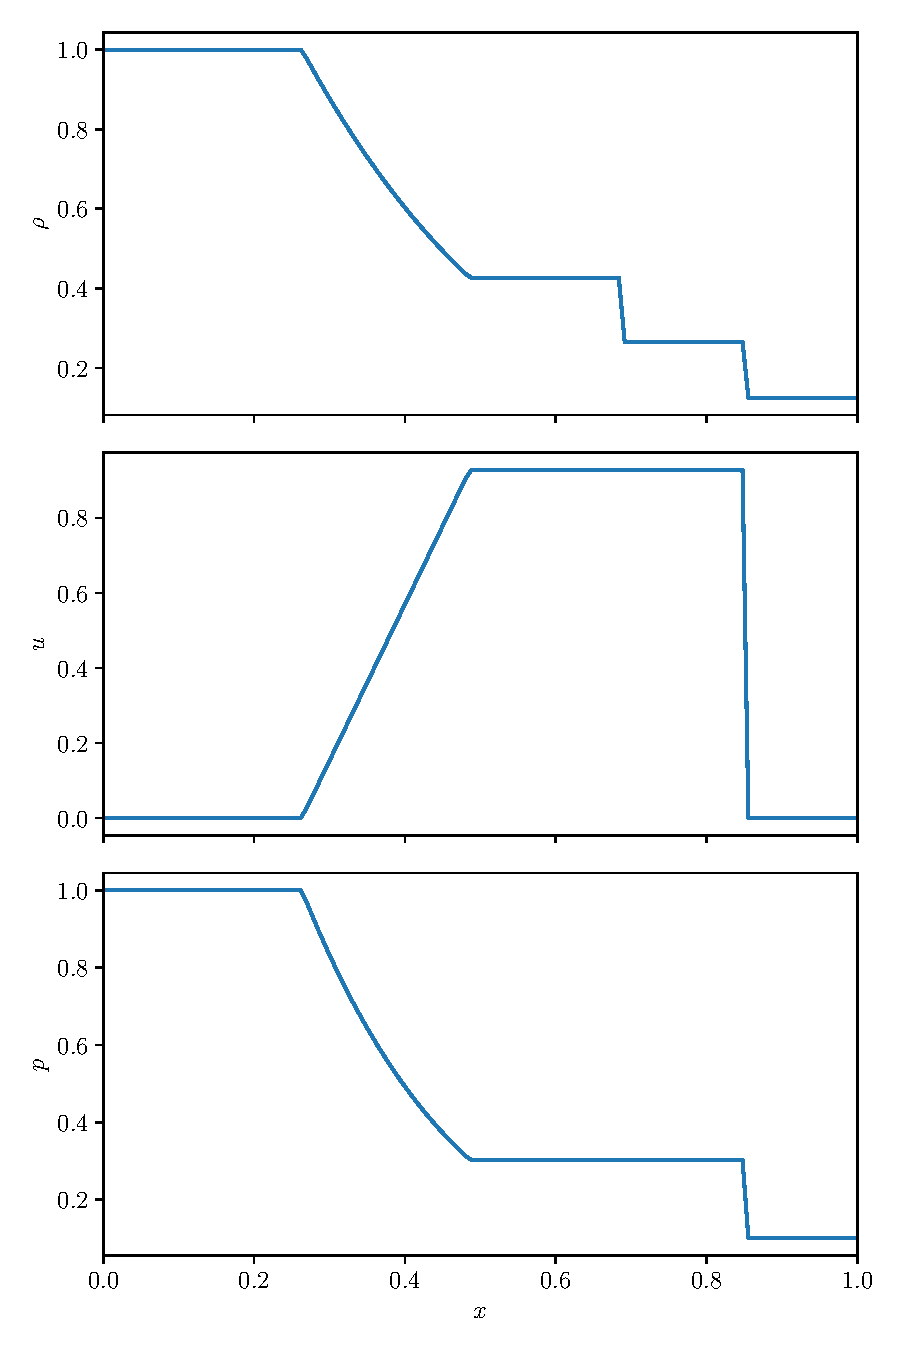
\includegraphics[width=0.8\linewidth]{riemann-sod}
\caption[The Sod problem]{\label{fig:sod} Evolution following from an initial
  discontinuity at $x = 0.5$.  These particular conditions are called
  the {\em Sod problem}, and in general, a setup with two states
  separated by a discontinuity is called a shock-tube problem.  We see three
  waves carrying changes in the solution. \\
  \hydroexdoit{\href{https://github.com/zingale/hydro_examples/blob/master/compressible/riemann-sod.py}{riemann-sod.py}}}
\end{figure}






%-----------------------------------------------------------------------------
\section{The Riemann problem}

\label{euler:sec:riemann}

Just like with advection and Burgers' equation, we will need to solve
a Riemann problem.  However, as our system is nonlinear, and has 3
waves, the solution is considerably more complex, but the general
ideas are straightforward.  Here we review the basic outline of
operations, and refer to Toro~\cite{toro:1997} for full details on a
variety of methods for solving the Riemann problem.

The Riemann problem consists of a left and right state separated by an
interface.  For the Euler equations, there are three eigenvalues,
which are the speeds at which information propagates.  Each of these
correspond to a wave that will move out from the interface with time,
and each wave will carry with it a jump in the characteristic
variables.  Figure~\ref{fig:riemann:waves} shows the
three waves moving out from the interface, separating space into 4
regions, marked: $L$, $L^*$, $R^*$, and $R$.
\begin{figure}[h]
\centering
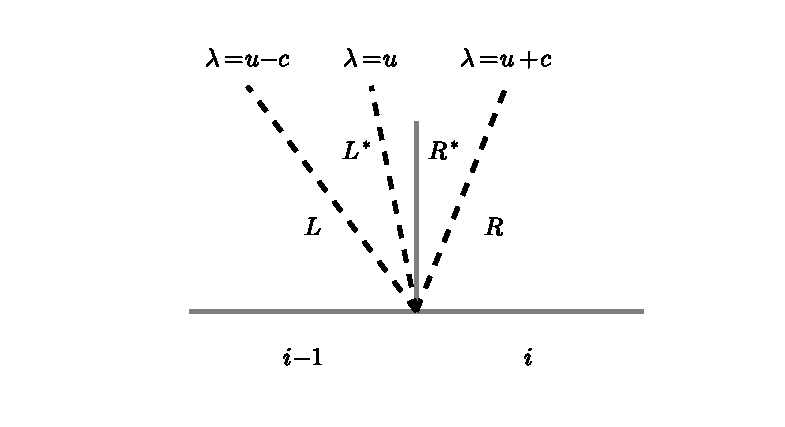
\includegraphics[width=\linewidth]{riemann-waves}
\caption[The Riemann problem wave structure for the Euler
  equations]{\label{fig:riemann:waves} The wave structure and 4
  distinct regions for the Riemann problem.  Time can be thought of as
  the vertical axis here, so we see the waves moving outward from the
  interface.}
\end{figure}
We typically work in terms of primitive variables.  The states in the
$L$ and $R$ regions are simply the left and right input states---the
waves have not had time to reach here, so they are unmodified.

Looking at the middle right eigenvector, $\rb^\evz$, we identify the
middle wave as a {\em contact discontinuity}.  There is neither
compression nor expansion across this wave (since the velocity does
not jump across it) and it simply separates two states.  We also know
from the eigenvectors that the pressure is constant across the
contact.

The left and right waves can be either a rarefaction or a shock.  It will
be a shock if the flow is compressing and a rarefaction otherwise.


\subsection{Rarefactions}

The conditions across a rarefaction can be understood by considering
a system where entropy replaces pressure, $\qb_s = (\rho, u, s)^\intercal$.
The entropy equation is simply $Ds/Dt = 0$.  We need to express the
pressure gradient in the velocity equation in terms of $\qb_s$.
\begin{equation}
\frac{\partial p(\rho, s)}{\partial x} =
  \left . \frac{\partial p}{\partial s} \right |_\rho \frac{\partial s}{\partial x} +
  \left . \frac{\partial p}{\partial \rho} \right |_s \frac{\partial \rho}{\partial x}
=
  \left . \frac{\partial p}{\partial s} \right |_\rho \frac{\partial s}{\partial x} +
  \frac{p\Gamma_1}{\rho} \frac{\partial \rho}{\partial x}
\end{equation}
giving
\begin{equation}
\frac{\partial u}{\partial t} + u \frac{\partial u}{\partial x} + \frac{1}{\rho} \left [
     \left . \frac{\partial p}{\partial s} \right |_\rho \frac{\partial s}{\partial x} +
          \frac{p\Gamma_1}{\rho} \frac{\partial \rho}{\partial x} \right ] = 0
\end{equation}
This gives a system:
\begin{equation}
{\qb_s}_t + \Ab_s(\qb_s) {\qb_s}_x = 0
\end{equation}
where
\begin{equation}
\Ab_s =
 \left ( \begin{array}{ccc} u & \rho & 0 \\
        c^2/\rho & u & \frac{1}{\rho} \left . \frac{\partial p}{\partial s}\right |_\rho \\
        0 & 0 & u \end{array} \right )
\end{equation}
The eigenvalues of $\Ab_s$ are again $u$, $u-c$, and $u+c$.  The right eigenvectors
are\footnote{Again, see the {\sf SymPy} {\sf Jupyter} notebook:
\hydroexdoit{\href{https://github.com/zingale/hydro_examples/blob/master/compressible/euler.ipynb}{euler.ipynb}}}
\begin{align}
\rb_s^\evm = \left ( \begin{array}{c} 1 \\ -c/\rho \\ 0 \end{array} \right )
%
\qquad
\rb_s^\evz = \left ( \begin{array}{c} 1 \\ 0 \\ -c^2/p_s  \end{array} \right )
%
\qquad
\rb_s^\evp = \left ( \begin{array}{c} 1 \\ c/\rho \\ 0 \end{array} \right )
\end{align}
Here, we define $p_s \equiv \partial p/\partial s |_\rho$.
Since the jump in $\qb_s$ is proportional to these eigenvectors, we see that
entropy does not change across the left, $(-)$, and right, $(+)$, waves.

Consider the $\evp$ wave, which moves at a speed $\lambda^\evp = u
+c$.  Across this wave, the characteristic variable $\wb^\evp$ will
jump, but the others will not.  Similarly, $\wb^\evp$ will be constant
across the $\evm$ wave.  So we can use this constancy to tell us how
the evolution behaves across that wave.  The constancy of the middle and right characteristic variables across the left
wave gives us the conditions (using our original primitive variable system):
\begin{align}
\lb^\evp \cdot d\qb &= 0 \\
\lb^\evz \cdot d\qb &= 0 
\end{align}
or 
\begin{equation}
\left ( \begin{array}{ccc} 0 & \frac{\rho}{2c} & \frac{1}{2c^2} \end{array} \right)
   \left ( \begin{array}{c} d\rho \\ du \\ dp \end{array} \right ) = 0
\qquad
%
\left ( \begin{array}{ccc} 1 & 0 & -\frac{1}{c^2} \end{array} \right)
   \left ( \begin{array}{c} d\rho \\ du \\ dp \end{array} \right ) = 0
\end{equation}
Expanding these, we have the system:
\begin{align}
du + \frac{1}{\rho c} dp &= 0 \\
d\rho - \frac{1}{c^2} dp &= 0 
\end{align}
Defining the {\em Lagrangian sound speed}, $C \equiv \rho c$, and the 
specific volume, $\tau = 1/\rho$, we can rewrite this system as:
\begin{equation}
du = -\frac{dp}{C} , \,\,\, d\tau = -\frac{dp}{C^2} \quad \mbox{across the left wave}
\end{equation}

Similar arguments would give the condition across the right wave as:
\begin{equation}
du = \frac{dp}{C} , \,\,\, d\tau = -\frac{dp}{C^2} \quad \mbox{across the right wave}
\end{equation}

These are completely general at this point.  Note that the condition
of the second wave, $d\tau/dp$ is essentially the definition of the
adiabatic index $\Gamma_1$, $dp/p - \Gamma_1 d\rho/\rho = 0$ for
constant entropy.  Finding the solution across the rarefaction then
involves integrating the system from $p_{l,r}$ to $p_\star$, where $l,
r$ is the original left or right state, depending on which wave you
are considering.  Coupled with this, we need our equation of state to
provide $C = C(\tau, p)$.  These solutions are called the {\em Riemann
  invariants}.

Considerable simplification can be made if we assume a gamma-law gas.
The eigensystem with entropy showed us that entropy is constant across
the solution.  This allows us to write our equation of state as:
\begin{equation}
p = K \rho^\gamma
\end{equation}
where $K$ is a constant that depends on the entropy, and do the 
integrals analytically.

\begin{exercise}[Riemann invariants for gamma-law gas]
Assume a gamma-law gas, then you only need to integrate a single
equation to find the solution across the left rarefaction:
\begin{equation}
u = - \int \frac{dp}{\rho c}
\end{equation}
where $c = \sqrt{\gamma p/\rho}$.  Using $p = K\rho^\gamma$, show that
\begin{equation}
u + \frac{2c}{\gamma - 1} = \mbox{constant} \quad \mbox{across the left rarefaction}
\end{equation}

This allows you to link the state to the left of the rarefaction to the star state:
\begin{equation}
u_l + \frac{2c_l}{\gamma - 1} = u_\star + \frac{2c_\star}{\gamma -1}
\end{equation}
and
\begin{equation}
\frac{p_l}{\rho_l^\gamma} = \frac{p_\star}{\rho_\star^\gamma}
\end{equation}
from our constant-entropy equation of state.  Together, show that this
gives:
\begin{equation}
u_{\star,l} = u_l + \frac{2c_l}{\gamma - 1} \left [ 1 - \left ( \frac{p_\star}{p_l}\right )^{(\gamma - 1)/2\gamma} \right ]
\end{equation}
A similar construction can be done for the right rarefaction, yielding:
\begin{equation}
u_{\star,r} = u_r - \frac{2c_r}{\gamma - 1} \left [ 1 - \left ( \frac{p_\star}{p_r}\right )^{(\gamma - 1)/2\gamma} \right ]
\end{equation}

\end{exercise}

For a general equation of state, there is not a closed form, but we would need
to integrate our system to get $u_\star = u(p_\star)$.

We'll denote the solution across the left rarefaction as $u_\star =
u_l^{rare}(p_\star)$ and across the right rarefaction as $u_\star =
u_r^{rare}(p_\star)$.

\subsection{Shocks}

Entropy is not constant across a shock---there is dissipation, so we
need a different way to connect the states across the shock.  As with
Burgers' equation, we can understand the shock by looking at the
Rankine-Hugoniot jump conditions.  There will be one condition for
each of our conservation laws, and together they tell us the speed of
the shock and how density and pressure jump across
it.  

The Rankine-Hugoniot conditions are:
\begin{equation}
\frac{\Fb(\Uc_\star) - \Fb(\Uc_s)}{\Uc_\star - \Uc_s} = S
\end{equation}
where $S$ is the shock speed.  It is easiest to work in the frame of the shock.  If the shock speed
is $S$, then we define the velocity in the shock frame as:
\begin{align}
\hat{u}_s &= u_s - S  \\
\hat{u}_\star &= u_\star - S
\end{align}
and the Rankine-Hugoniot conditions become:
\begin{equation}
\frac{\Fb(\hat{\Uc}_\star) - \Fb(\hat{\Uc}_s)}{\hat{\Uc}_\star - \hat{\Uc}_s} = 0
\end{equation}

For the one-dimensional system of Euler equations, we have the conditions:
\begin{align}
\rho_\star \hat{u}_\star &= \rho_s \hat{u}_s \\
\rho_\star \hat{u}_\star^2 + p_\star &= \rho_s \hat{u}_s^2 + p_s \\
\rho_\star \hat{u}_\star e_\star + \frac{1}{2} \rho_\star \hat{u}_\star^3 + \hat{u}_\star p_\star &= 
  \rho_s \hat{u}_s e_s + \frac{1}{2} \rho_s \hat{u}_s^3 + \hat{u}_s p_s
\end{align}
Our goal is to find how each variable jumps across the shock.  We'll 
work this out for the general EOS case, following the ideas in \cite{colellaglaz:1985}.

Starting with the mass flux, we can express:
\begin{equation}
\hat{u}_\star = \frac{\rho_s}{\rho_\star} \hat{u}_s
\end{equation}
and then insert this into the momentum equation to get:
\begin{equation}
\rho_s^2 \left ( \frac{1}{\rho_s} - \frac{1}{\rho_\star} \right ) \hat{u}_s^2 = p_\star - p_s
\end{equation}
Introducing compact notation for the jump across the shock:
\begin{equation}
[q] \equiv q_\star - q
\end{equation}
we have:
\begin{equation}
-[\tau] = \frac{[p]}{\rho_s^2 \hat{u}_s^2}
\end{equation}

We now introduce the mass flux, $W_s$.  For a shock separating
$L$/$L\star$ (the 1-shock), mass will be moving through the shock to the
right, so, in the frame of the shock, the mass flux is
\begin{equation}
W_L \equiv \rho_L \hat{u}_L = \rho_\star \hat{u}_\star
\end{equation}
Likewise, for a shock separating $R$/$R\star$ (the 3-shock), mass will
move to the left passing through the shock, and in the frame of the
shock, the mass flux is
\begin{equation}
W_R \equiv -\rho_R \hat{u}_R = -\rho_\star \hat{u}_\star
\end{equation}

Thus, our first jump condition becomes
\begin{equation}
-[\tau] = \frac{[p]}{W_s^2}
\end{equation}

Next, going back to the momentum equation, we can substitute in the
mass flux.  For the left (1-shock), we have:
\begin{equation}
W_L \hat{u}_\star + p_\star = W_L \hat{u}_L + p_L
\end{equation}
giving
\begin{equation}
[u] = -\frac{[p]}{W_L}
\end{equation}
where we recognized that $\hat{u}_\star - \hat{u}_L = u_\star - u_L =
[u]$, since the shock speed is the same for $u_\star$ and $u$.

Likewise, for the right (3-shock), we have:
\begin{equation}
-W_R \hat{u}_\star + p_\star = -W_R \hat{u}_R + p_R
\end{equation}
giving
\begin{equation}
[u] = \frac{[p]}{W_R}
\end{equation}

The last jump condition is for energy.  Since all the terms in the 
energy equation are proportional to velocity, there will be no sign
difference between the left and right shock jump conditions.  
We start by introducing the mass flux:
\begin{equation}
W_s e_\star + \frac{1}{2} W_s \hat{u}_\star^2 + \frac{W_s}{\rho_\star} p_\star =
  W_s e_s + \frac{1}{2} W_s \hat{u}_s^2 + \frac{W_s}{\rho_s} p_s
\end{equation}
The mass flux cancels, leaving
\begin{equation}
[e] + \frac{p_\star}{\rho_\star} - \frac{p_s}{\rho_s} + \frac{1}{2} \left ( \hat{u}_\star^2 - \hat{u}_s^2 \right ) = 0
\end{equation}
getting rid of the velocities using $\hat{u}_\star^2 = W_s^2/\rho_\star^2$ and 
$\hat{u}_s^2 = W_s^2/\rho_s^2$, we have:
\begin{equation}
[e] + \frac{p_\star}{\rho_\star} - \frac{p_s}{\rho_s} + \frac{1}{2} W_s^2 \left ( \frac{1}{\rho_\star^2} - \frac{1}{\rho_s^2} \right ) = 0
\end{equation}
Then introducing $W_s^2 = -[p]/[\tau]$, and after a lot of algebra, we arrive at:
\begin{equation}
[e] = -\frac{p_\star + p_s}{2} [\tau]
\end{equation}
Some sources write $\bar{p} \equiv (p_\star + p_s)/2$.

To summarize, our jump conditions across the shock are:
\begin{align}
[\tau] &= -\frac{[p]}{W_s^2} \\
[u] &= \mp \frac{[p]}{W_s} \quad\mbox{`$-$' for left, `+' for right}\\
[e] &= - \frac{p_\star + p_s}{2} [\tau] \label{eq:euler:shock:ejump}
\end{align}

As with the rarefaction, the goal is to express this as a function, $u_\star
= u_s^\mathrm{shock}(p_\star)$.  The general solution procedure is starts with
a proposed value for $p_\star$, then:
\begin{enumerate}
\item root find to find $\rho_\star$ corresponding to the $p_\star$:
  \begin{enumerate}
  \item guess a value for $\rho_\star$
  \item using the equation of state, express $e_\star = e(p_\star, \rho_\star)$
  \item use Newton's method (or another technique) with $[e] = -\bar{p} [\tau]$
     to find a correction to $\rho_\star$
  \end{enumerate}
\item compute 
  \begin{equation}
    \frac{1}{W_s^2} = - \frac{[\tau]}{[p]}
  \end{equation}
\item find the star velocity:
  \begin{equation}
    u_\star = u_s \mp \frac{[p]}{W_s}
  \end{equation}
  where we use `$-$' for the left shock, and `+' for the right shock
\end{enumerate}

The one other piece of information we need is the shock speed.  We can
get this from the mass flux, $W_s$, definition, e.g., $W_L = \rho_L
\hat{u}_L = \rho_L (u_L - S)$,:
\begin{equation}
S = u_s \mp \frac{W_s}{\rho_s} \quad\mbox{`$-$' for left, `+' for right}\\
\end{equation}

Just as with the rarefaction, considerable simplification can be made if 
we assume a gamma-law gas.

\begin{exercise}[Shock jump conditions for $\gamma$-law EOS]
{
Introducing 
\begin{equation}
e = \frac{p}{\rho} \frac{1}{\gamma -1}
\end{equation}
into the jump condition for energy, Eq.~\ref{eq:euler:shock:ejump},
show that we can express the jump in density in terms of the
ratio of pressure, $p_\star/p_s$, as:
\begin{equation}
\label{eq:euler:shockrhojump}
\rho_\star = \rho_s \left [ \frac{ \frac{p_\star}{p_s} (\gamma + 1) + (\gamma - 1)}
   {(\gamma + 1) + \frac{p_\star}{p_s} (\gamma -1)} \right ]
\end{equation}
}

Now, compute the mass flux, $W_s$ starting with
\begin{equation}
W_s^2 = -\frac{[p]}{[\tau]}
\end{equation}
use the $\gamma$-law equation of state and show that
\begin{equation}
W_s^2 = \frac{1}{2} p_s \rho_s \left [ \left(\frac{p_\star}{p_s}\right) (\gamma + 1) + (\gamma -1) \right ]
\end{equation}

With this, show that the star velocity is:
\begin{equation}
\label{eq:euler:shockujump}
u_\star = u_s \pm c_s \left [\frac{2}{\gamma(\gamma - 1)}\right]^{1/2} \frac{1 - \frac{p_\star}{p_s}}{\left ( \frac{p_\star}{p_s} \frac{\gamma + 1}{\gamma - 1} + 1\right)^{1/2}}
\end{equation}
with `+` for the left shock and `$-$` for the right shock.
Also show that the shock speed is:
\begin{equation}
\label{eq:euler:shockspeedjump}
S = u_s \mp c_s \left [ \left ( \frac{p_\star}{p_s} \right ) \frac{\gamma+1}{2\gamma} + \frac{\gamma-1}{2\gamma} \right ]^{1/2}
\end{equation}
with the `$-$' or the left shock and the `+' for the right shock.
\end{exercise}
  
\subsection{Finding the Star State}

The left and right states are connected to the state in the star
region by a Hugoniot curve---this is a curve in the $u$-$p$ plane that
shows all of the possible states one can reach from the current state
through either a shock or rarefaction.  There are two such curves, one
corresponding to the left and one to the right state:
\begin{equation}
u_{\star,l}(p) = \begin{cases}
   u_{\star,l}^\mathrm{shock}(p) & p > p_l \\
   u_{\star,l}^\mathrm{rare}(p) & p \le p_l 
   \end{cases}
\qquad
u_{\star,r}(p) = \begin{cases}
   u_{\star,r}^\mathrm{shock}(p) & p > p_r \\
   u_{\star,r}^\mathrm{rare}(p) & p \le p_r 
   \end{cases}
\end{equation}
The solution
to the Riemann problem is the point in the $u$-$p$ plane where these
two curves intersect, e.g., we solve for $p_\star$ in:
\begin{equation}
u_{\star,l}(p_\star) - u_{\star,r}(p_\star) = 0
\end{equation}
This is equivalent to saying that pressure and velocity do not jump
across the contact wave.

For a gamma-law equation of state, using the results from the
exercises, we have:
\begin{equation}
\renewcommand{\arraystretch}{1.5}
u_{\star,s}(p_\star) = \begin{cases}
  u_s \pm \frac{2c_s}{\gamma - 1} \left [ 1 - \left ( \frac{p_\star}{p_s}\right )^{(\gamma - 1)/2\gamma} \right ] & p_\star \le p_s \\
\\
%
  u_s \pm c_s \left [\frac{2}{\gamma(\gamma - 1)}\right]^{1/2} \frac{1 - \frac{p_\star}{p_s}}{\left ( \frac{p_\star}{p_s} \frac{\gamma + 1}{\gamma - 1} + 1\right)^{1/2}} & p_\star > p_s
\end{cases}
\renewcommand{\arraystretch}{1.0}
\end{equation}



Figure~\ref{fig:euler:riemann-curve} shows the Hugoniot curves for the
Sod problem.  Comparing to Figure~\ref{fig:sod}, we see that the right
state is linked to the star state with a shock while the left state is
linked to the star state with a rarefaction.

\begin{exercise}[Hugoniot curves]
Download the code demonstrated in Figure~\ref{fig:euler:riemann-curve}
and experiment with different initial conditions to see how the
solution changes based on the states.  Try to create initial states
that give rise to two rarefactions and a separate set of states that
give rise to two shocks.
\end{exercise}

\begin{figure}[t]
\centering
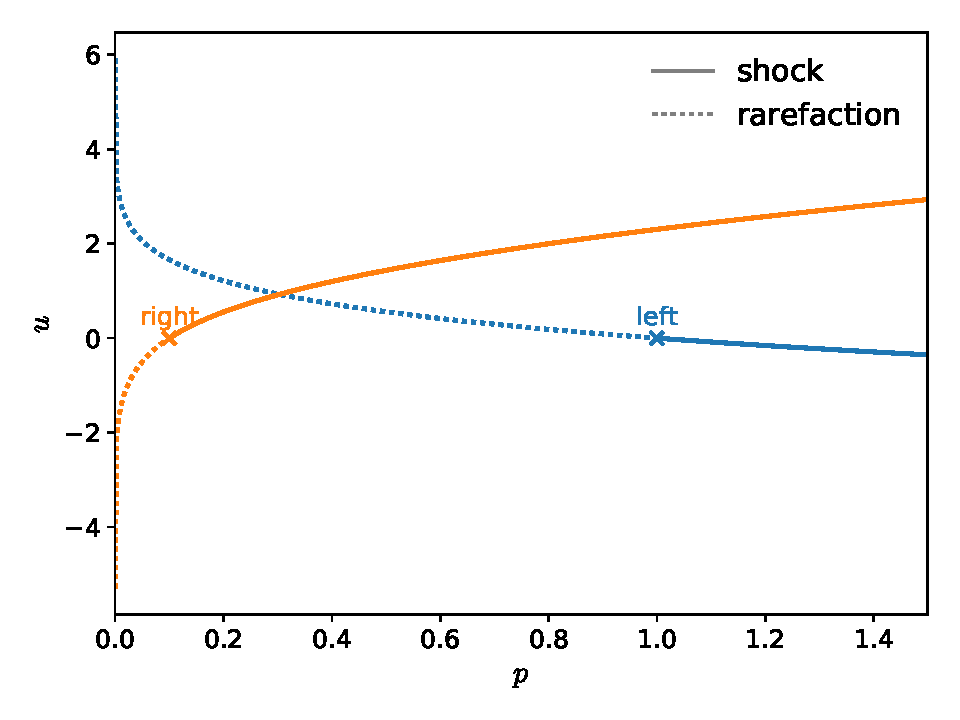
\includegraphics[width=0.9\linewidth]{riemann-phase}
\caption[The Hugoniot curves corresponding
to the Sod problem]{\label{fig:euler:riemann-curve} The Hugoniot
curves corresponding to the Sod problem.  The shock and rarefaction
curves are shown.  The solution to the Riemann problem is the point
where the curves intersect.  The line style of the curve indicates
where we are a shock or rarefaction.  Where $p > p_s$, where $s \in {L,R}$, we have a shock.\\
\hydroexdoit{\href{https://github.com/zingale/hydro_examples/blob/master/compressible/riemann-phase.py}{riemann-phase.py}}}
\end{figure}


\subsection{Complete Solution}

To complete the solution, we need to find which of the 4 regions, $L,
L\star, R\star, R$ we fall in.  For hydrodynamics, we are usually
interested only in the solution on the interface, but we can look
along any ray in the $x$-$t$ plane by defining $\xi = (x -
x_\mathrm{interface})/t$.  If the initial discontinuity is on the
interface, then $\xi = 0$.

\begin{figure}
\centering
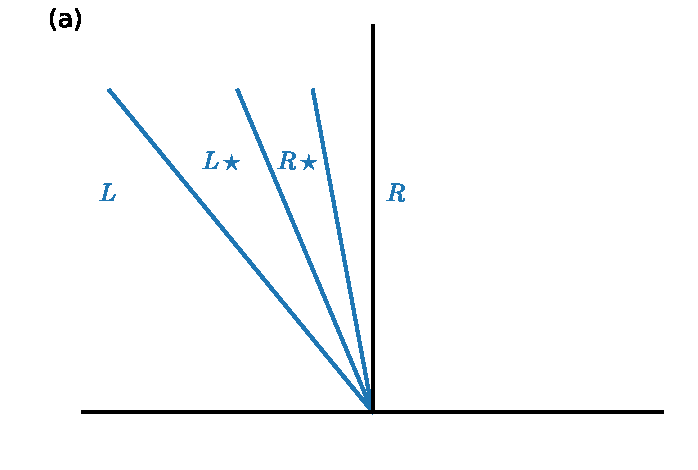
\includegraphics[width=0.49\linewidth]{riemann_waves_ifc_R}
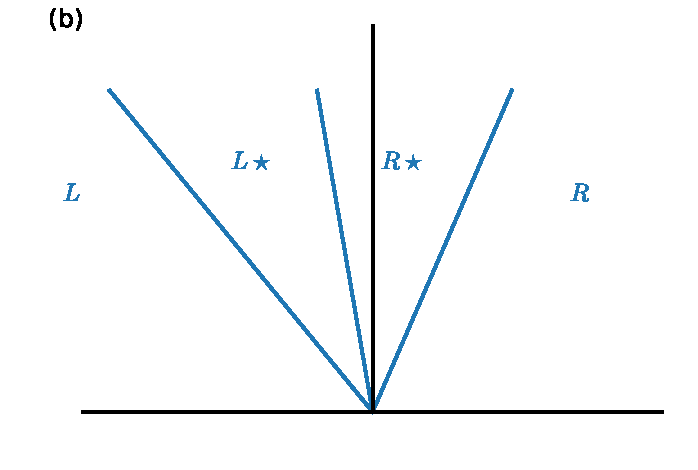
\includegraphics[width=0.49\linewidth]{riemann_waves_ifc_Rstar} \\
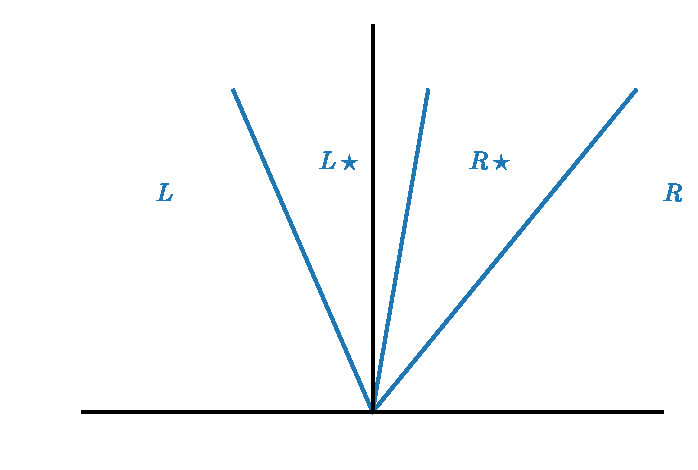
\includegraphics[width=0.49\linewidth]{riemann_waves_ifc_Lstar}
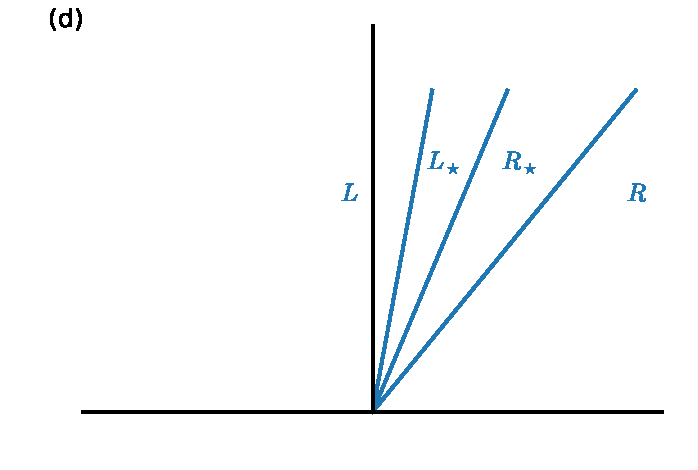
\includegraphics[width=0.49\linewidth]{riemann_waves_ifc_L} 
\caption[Wave configuration for the Riemann problem]
        {\label{fig:euler:riemann_sample} An illustration of the 3
          waves emanating from an initial discontinuity (the origin of
          the axes).  The 4 cases show all possible cases of waves
          being to the left or right of the interface (corresponding
          to the choice $\xi = 0$).  In all cases, the middle wave is
          a contact and the left (1) and right (3) waves are either a
          shock or a rarefaction.  The state on the interface is: $R$
          (case a); $R\star$ (case b); $L\star$ (case c); $L$ (case
          d).}
\end{figure}

Figure~\ref{fig:euler:riemann_sample} shows the possible
configurations of the waves.  Note that the middle wave is always a
contact but the left (1) and right (3) waves can be either a shock or
rarefaction.  To find out which region the interface falls in, we simply
look at the speeds.  

The first speed to consider is the contact wave, that has a speed of
simply $S_c = u_\star$.  If $S_c > \xi$, then we are choosing between
the $L$ and $L_\star$ states (cases c and d in
Figure~\ref{fig:euler:riemann_sample}).  If $S_c < \xi$, then we are
choosing between $R$ and $R_\star$ states (cases a and b).

This will leave just a single wave to consider: the right wave for
cases a and b; and the left wave for cases c and d.  We need the wave
speed for this---it will depend on whether it is a shock or a
rarefaction.



%-----------------------------------------------------------------------------
\section{Other thermodynamic equations}

At times we will want to use alternate forms of the energy equation.  The
internal energy is governed by the first law of thermodynamics.  In the
absence of any heat sources, we have:
\begin{equation}
dq = 0 = de + pd(1/\rho)
\end{equation}
where $e$ is the specific internal energy.
Applying this to a Lagrangian fluid element, we have:
\begin{align}
\DDt{e} + p \DDt{(1/\rho)} &= 0 \\
\DDt{e} - \frac{p}{\rho^2} \frac{D\rho}{Dt} &= 0 \\
\rho \frac{De}{Dt} + p \nabla \cdot \Ub &= 0
\end{align}
where we used the continuity equation in the last step to eliminate
$D\rho/Dt$.  This can be rewritten by adding $e \times$ the continuity
equation to give:
\begin{equation}
\ddt{(\rho e)} + \nabla \cdot (\rho \Ub e) + p \nabla \cdot \Ub = 0 \label{eq:euler:econs}
\end{equation}

Notice that internal energy, $(\rho e)$ is not a conserved quantity
(in particular, the $p\nabla \cdot \Ub$ term is not in conservative
form).  

Another energy-like quantity that we can consider is specific enthalpy,
\begin{equation}
h = e + \frac{p}{\rho}
\end{equation}
Differentiating this, and using the internal energy equation,
\begin{align}
\DDt{h} &= \DDt{e} - \frac{p}{\rho^2} \DDt{\rho} + \frac{1}{\rho} \DDt{p} \\
        &= \frac{p}{\rho^2}\DDt{\rho} - \frac{p}{\rho^2} \DDt{\rho} + \frac{1}{\rho} \DDt{p}
\end{align}
so
\begin{equation}
\rho \DDt{h} = \DDt{p}
\end{equation}

This form is useful for very subsonic flows (see,
e.g.~\cite{SNpaper}), where $Dp/Dt = 0$, which then shows that
enthalpy is conserved:
\begin{equation}
\ddt{(\rho h)} + \nabla \cdot (\rho h \Ub) = 0
\end{equation}
(here we added $h \times$ the continuity equation to transform from
the Lagrangian derivative to a conservation equation).


We can also look at the temperature evolution.  It is interesting to
approach this from both the internal energy and enthalpy equations.
Starting with internal energy, writing it as $e(\rho, T)$, we have:
\begin{equation}
\DDt{e} = \left . \frac{\partial e}{\partial \rho} \right |_T \DDt{\rho} +
          \left . \frac{\partial e}{\partial T} \right |_\rho \DDt{T} = -\frac{p}{\rho} \nabla \cdot \Ub
\end{equation}
The specific heat at constant volume is defined as $c_v = \partial
e/\partial T|_\rho$, allowing us to write:
\begin{equation}
c_v \DDt{T} = \left ( \left . \frac{\partial e}{\partial \rho} \right |_T - \frac{p}{\rho} \right ) \nabla \cdot \Ub
\end{equation}

If we alternately start with enthalpy, expressing it as $h = h(p, T)$,
we have:
\begin{equation}
\DDt{h} = \left . \frac{\partial h}{\partial p} \right |_T \DDt{p} +
          \left . \frac{\partial h}{\partial T} \right |_p \DDt{T} = \frac{1}{\rho} \DDt{p}
\end{equation}
The specific heat at constant pressure is defined as $c_p = \partial
h/\partial T|_p$, letting us write:
\begin{equation}
c_p \DDt{T} = \left ( \frac{1}{\rho} - \left . \frac{\partial h}{\partial p} \right |_T \right ) \DDt{p}
\end{equation}

These two temperature evolution equations are equivalent, but one
describes the evolution in terms of density and the other in terms of
pressure.  Later, we'll see how these can be useful when we
approximate the evolution of reactive flow under constant density or
constant pressure behaviors.

\if debug
\subsection{Eigensystem with temperature}

Here we illustrate how the eigensystem changes when we replace pressure with
temperature in our primitive variable system.

We write this set of variables as $\hat{\qb} = (\tau, u,
T)^\intercal$---note that we keep $\tau$ instead of $\rho$ here.  The
motivation for this comes from the fact that with temperature in the
mix, the temperature will jump across the contact wave.  Since
pressure should be constant across the contact, and, even with the
general EOS, a temperature jump needs a density drop for pressure to
remain constant, $\tau$ should counteract the behavior of $T$ across
the contact.

The temperature evolution equation appears as:
\begin{equation}
\frac{\partial T}{\partial t} = -u\ddx{T} +
  \frac{1}{\rho c_p} \left [ (1 - \rho h_p) \frac{Dp}{Dt} \right ]
\end{equation}
(see, e.g.\ \cite{ABRZ:I}) where $c_p$ is the specific heat at
constant pressure, $c_p = \partial h/\partial T|_p$ and $h_p \equiv
\partial h / \partial p |_T$, with $h = e + p/\rho$ the specific
enthalpy.  We can use the standard pressure evolution equation
(Eq.~\ref{eq:euler:pgeneral}) to eliminate the Lagrangian pressure term,
resulting in:
\begin{equation}
\frac{\partial T}{\partial t} = -u\ddx{T} - \eta \ddx{u}
\end{equation}
where we defined
\begin{equation}
\eta \equiv \frac{1 - \rho h_p}{c_p} c^2
\end{equation}

The density equation remains unchanged from the traditional primitive
variable formulation, but for the velocity, we need to write the
$\partial p/\partial x$ term in terms of $\hat{\qb}$.  We do this via
the chain rule.  We define $p_\rho \equiv {\partial p}/{\partial \rho}
|_T$ and $p_T \equiv {\partial p}/{\partial T} |_\rho$, then our
velocity equation is:
\begin{equation}
\frac{\partial u}{\partial t} + u \frac{\partial u}{\partial x} - \frac{p_\rho}{\tau} \frac{\partial \tau}{\partial x} + {\tau p_T} \frac{\partial T}{\partial x} = 0
\end{equation}
Note that here we neglected any composition dependence in the EOS.

Our primitive variable system in matrix form is then:
\begin{equation}
\hat{\qb}_t + \hat{\Ab} \hat{\qb}_x = 0
\end{equation}
with
\begin{equation}
\renewcommand{\arraystretch}{1.5}
\hat{\Ab}(\hat{\qb}) =
\left (
\begin{array}{ccc}
u                   & -\tau & 0 \\
-\dfrac{p_\rho}{\tau} & u    & \tau p_T \\
0                   & \eta & u
\end{array}
\right )
\end{equation}
The eigenvalues can be found through the characteristic polynomial,
$|\hat{\Ab} - \lambda I| = 0$:
\begin{equation}
(u - \lambda)^3 - (u -\lambda) \left ( {p_T \eta\tau} + p_\rho \right ) = 0
\end{equation}
We can simplify the last term in parenthesis:
\begin{equation}
{p_T \eta\tau} + p_\rho = \frac{p_T (1 - \rho h_p) c^2}{\rho c_p} + p_\rho
                               = \frac{c^2}{c_p}\left ( \frac{p p_T}{\rho^2 p_\rho} - \frac{p_T e_\rho}{p_\rho} \right ) + p_\rho \label{eq:step1}
\end{equation}
where we substituted in
\begin{equation}
h_p = \frac{1}{\rho} \left ( 1 - \frac{p}{\rho p_\rho} \right ) + \frac{e_\rho}{p_\rho}
\end{equation}
(see \cite{ABRZ:I}, appendix A) where $e_\rho = \partial e/\partial
\rho |_T$.  The term in parenthesis in Eq.~\ref{eq:step1} is simply
$c_p - c_v$ (\cite{cg}, Eq.~9.81) where $c_v$ is the specific heat
at constant volume, and Eq.~\ref{eq:step1} further reduces to:
\begin{equation}
{p_T \eta\tau} + p_\rho = \frac{c^2}{c_p} (c_p - c_v) + p_\rho
                               = c^2 - c^2 \frac{\chi_p}{\Gamma_1} + p_\rho = c^2
\end{equation}
where we used $c_v/c_p = \chi_p/\Gamma_1$ and $\chi_p = \rho p_\rho /
p$ (\cite{cg}, Eqs.~9.87, 9.82).  Putting this into our
characteristic polynomial, we see that the eigenvalues are, as expected,
$\lambda = u, u \pm c$.  It is also useful to note that
\begin{equation}
\eta = \frac{c^2 - p_\rho}{\tau p_T}
\end{equation}


We construct the left and right eigenvectors such that they are orthonormal,
and find:
\begin{equation}
\renewcommand{\arraystretch}{1.3}
\hat{R} = \left ( \begin{array}{ccc}
     1                       & 1                 & 1 \\
   c/\tau                    & 0                 & -c/\tau \\
  -(c^2 - p_\rho)/\tau^2 p_T & p_\rho/\tau^2 p_T & -(c^2 - p_\rho)/\tau^2 p_T
  \end{array} \right )
\end{equation}
and
\begin{equation}
\hat{L} = \left ( \begin{array}{ccc}
      {p_\rho}/{2 c^2}   & {\tau}/{2c}  & -{\tau^2 p_T}/{2 c^2} \\
      1 - {p_\rho}/{c^2} &0             & {\tau^2 p_T}/{c^2} \\
      {p_\rho}/{2 c^2}   & -{\tau}/{2c} & -{\tau^2 p_T}/{2 c^2} \end{array} \right )
\end{equation}
We note that all
thermodynamic derivatives are expressed in terms of $\rho$ or $T$ with
the other quantity held constant.  This is in the form we expect a
$(T, \rho)$-based EOS to return derivatives.  Notice also that the
temperature jumps across the $\evz$ wave (the contact discontinuity;
this is seen from the non-zero value in $\hat{r}^\evz$ for the
temperature).

We write:
\begin{eqnarray}
\hat{\beta}^\evm_s &\equiv& (\hat{l}^\evm \cdot \Delta \hat{\qb}^\evm ) =
   \frac{1}{2C} \left (\frac{\rho^2 p_\rho}{C} \Delta \tau^\evm
                        + \Delta u^\evm - \frac{p_T}{C}\Delta T^\evm \right ) \\
%
\hat{\beta}^\evz_s &\equiv& (\hat{l}^\evz \cdot \Delta \hat{\qb}^\evz ) =
    \Delta \tau^\evz +
        \frac{1}{C^2} \left (-\rho^2 p_\rho \Delta \tau^\evz
                        + {p_T}\Delta T^\evz \right ) \\
%
\hat{\beta}^\evp_s &\equiv& (\hat{l}^\evp \cdot \Delta \hat{\qb}^\evp ) =
   \frac{1}{2C} \left (\frac{\rho^2 p_\rho}{C} \Delta \tau^\evp
                        - \Delta u^\evp - \frac{p_T}{C}\Delta T^\evp \right )
\end{eqnarray}
Note that since $p_\tau = -\rho^2 p_\rho$, we can form a $\Delta p^\enu$ as
\begin{equation}
\Delta p^\enu = p_\tau \Delta \tau^\enu + p_T \Delta T^\enu
\end{equation}
and then we see that the $\hat{\beta}^\enu$'s above have the same
functional form as the $\mathring{\beta}^\enu$ from the $\mathring{\qb}
= (\tau, u, p, e)^\intercal$ eigensystem.  This is no surprise, since
the $l\cdot \Delta \qb$ are the characteristic variables of the Euler
equations.  The numerical values will differ though, because the
$\hat{\beta}^\enu$ and $\mathring{\beta}^\enu$ use different reference
states and reconstructed variables.

Finally, we can write out the interface states:
\begin{eqnarray}
\tau_s &=& \tilde{\tau} - (\hat{\beta}^\evm + \hat{\beta}^\evz + \hat{\beta}^\evp) \\
%
u_s &=& \tilde{u} - (C \hat{\beta}^\evm - C \hat{\beta}^\evp) \\
%
T_s &=& \tilde{T} - \frac{1}{p_T} \left \{
   \left [ -C^2 \hat{\beta}^\evm - C^2 \hat{\beta}^\evp \right ] +
   \rho^2 p_\rho \left [ \hat{\beta}^\evm + \hat{\beta}^\evz + \hat{\beta}^\evp \right ] \right \}
\end{eqnarray}
For $T_s$, we recognize the first quantity in the square brackets as
being the same as $-(p_s - \tilde{p})$ in the $\mathring{\qb}$ system, and the
second term in the square brackets being the same as $-(\tau_s - \tilde{\tau})$
in the $\mathring{\qb}$ system, then we see
\begin{equation}
p_T (T_s - \tilde{T} ) \approx (p_s - \tilde{p} ) - p_\tau (\tau_s - \tilde{\tau})
\end{equation}
which is what we would expect for jumps in $p$ when applying the chain
rule.  Note that this is not a strict equality, since the reference
states and interpolation between the two eigensystems are different.
Nevertheless, this demonstrates the connection between the two
methods.

The above did not consider variations in the composition of the fluid.
Multiple species complicate things---now the replacement of the
pressure gradient picks up a composition gradient term.
The eigensystem will change with this addition.  We don't explore this here at this
time.
\fi

